\documentclass{article}

\usepackage{url}
\usepackage{tikz}
\usepackage{float}
\usepackage{amsmath}
\usepackage{enumitem}

\usetikzlibrary{matrix, shapes, snakes, arrows}
\tikzset{>=triangle 45}

\title{CS 610: Midterm\\Winter 2013}

\author{Dustin Ingram}

\date{\today}

\begin{document}

\maketitle

\begin{enumerate}[start=0]

\item{} % 1

\begin{enumerate}

\item{} % a
    We consider three probabilities:
\begin{itemize}
    \item{The probability of being in the initial start state, $S_0$, where:}
    \begin{align*}
        S_0 &= \text{(\texttt{LanguageA}/Anti-Polka)}\\
        P_0 &= 0.7 \cdot 0.6 = 0.42
    \end{align*}
    \item{The probability of a transition from $S_0$ to $S_1$, where:}
    \begin{align*}
        S_1 &= \text{(\texttt{LanguageB}/Anti-Polka)}\\
        P_1 &= 0.15 \cdot 0.7 = 0.105
    \end{align*}
    \item{The transition from $S_1$ to $S_2$, where:}
    \begin{align*}
        S_1 &= \text{(\texttt{LanguageC}/Dummy)}\\
        P_1 &= 0.7 \cdot 0.3 = 0.21
    \end{align*}
\end{itemize}
Thus, the probability that \emph{at the beginning of the day} the machine will
produce chips in the order $S_0 \to S_1 \to S_2$ is:
\begin{align*}
    P_0 \cdot P_1 \cdot P_2 &= 0.42 \cdot 0.105 \cdot 0.21\\
    &= 0.009261\\
    &\approx 1\%
\end{align*}
\item{}
    We consider the first, heavy TV. For simplicity, we use the following
    notation:
    \begin{align*}
    P(C|W_h) &= P(\text{chip}_1, \text{chip}_2 | \text{weight} = \text{heavy})\\
    P(W_h|C) &= P(\text{weight} = \text{heavy} | \text{chip}_1, \text{chip}_2)\\
    P(W_h) &= P(\text{weight}=\text{heavy})\\
    P(C_s) &= P_{start}(\text{chip}_1, \text{chip}_2)
    \end{align*}
    The probability for the chips at the start of the run, $P(C_s)$ is given in
    part (a) and is as follows:
    \begin{figure}[H]
    \centering
    \begin{tabular}{|c||c|c|c|}
        \hline
        & \texttt{LanguageA} & \texttt{LanguageB} & \texttt{LanguageC}
        \\\hline\hline
        Anti-Polka & 0.42 & 0.14 & 0.14 \\\hline
        Dummy & 0.18 & 0.06 & 0.06 \\\hline
    \end{tabular}
    \end{figure}
    We are given $P(W_h|C)$ by the table in the question. $P(W_h)$ is given as
    follows:
    \begin{align*}
        P(W_h) = \sum{\left( P(W_h|C)\cdot P(C_s)\right)} = \textbf{0.486}
    \end{align*}
    Using Bayes' theorem:
    $$ P(C|W_h) = \frac{P(W_h|C) \cdot P(C_s)}{P(W_h)} $$
    Thus, the resulting values for $P(C|W_h)$ for the first, heavy TV are as follows:
    \begin{figure}[H]
    \centering
    \begin{tabular}{|c||c|}
        \hline
        $P(\text{Anti-Polka},\text{\texttt{LanguageA}}|\text{weight}=\text{heavy})$
        & \textbf{0.60} \\\hline
        $P(\text{Anti-Polka},\text{\texttt{LanguageB}}|\text{weight}=\text{heavy})$
        & \textbf{0.14}\\\hline
        $P(\text{Anti-Polka},\text{\texttt{LanguageC}}|\text{weight}=\text{heavy})$
        & \textbf{0.12}\\\hline
        $P(\text{Dummy},\text{\texttt{LanguageA}}|\text{weight}=\text{heavy})$ &
        \textbf{0.11}\\\hline
        $P(\text{Dummy},\text{\texttt{LanguageB}}|\text{weight}=\text{heavy})$ &
        \textbf{0.01}\\\hline
        $P(\text{Dummy},\text{\texttt{LanguageC}}|\text{weight}=\text{heavy})$ &
        \textbf{0.01}\\\hline
    \end{tabular}
    \end{figure}
    For the second, light TV, we use the following
    \begin{align*}
    P(C|W_l) &= P(\text{chip}_1, \text{chip}_2 | \text{weight} = \text{light})\\
    P(W_l|C) &= P(\text{weight} = \text{light} | \text{chip}_1, \text{chip}_2)\\
    P(W_l) &= P(\text{weight}=\text{light})\\
    P(C_t) &= P_{transition}(\text{chip}_1, \text{chip}_2)
    \end{align*}

    We no longer need to consider the probabilities of the starting state, but
    rather the transition between any two states:
    \begin{figure}[H]
    \centering
    \begin{tabular}{|c||c|c|c|c|c|c|}
        \hline
            & AP, \texttt{LA} &
            AP, \texttt{LB}&
            AP, \texttt{LC}&
            D, \texttt{LA}&
            D, \texttt{LB}&
            D, \texttt{LC}\\\hline\hline
            AP, \texttt{LA}&
            0.490 & 0.105 & 0.105 & 0.210 & 0.045 & 0.045\\\hline
            AP, \texttt{LB}&
            0.105 & 0.490 & 0.105 & 0.045 & 0.210 & 0.045\\\hline
            AP, \texttt{LC}&
            0.105 & 0.105 & 0.490 & 0.045 & 0.045 & 0.210\\\hline
            D, \texttt{LA}&
            0.210 & 0.045 & 0.045 & 0.490 & 0.105 & 0.105\\\hline
            D, \texttt{LB}&
            0.045 & 0.210 & 0.045 & 0.105 & 0.490 & 0.105\\\hline
            D, \texttt{LC}&
            0.045 & 0.045 & 0.210 & 0.105 & 0.105 & 0.490\\\hline
    \end{tabular}
    \end{figure}
    However, this probability of transition is assuming that we are equally
    likely to be in any given preceding state. As we have shown in the first
    half of the question where the first TV is heavy, in this case there is a
    known probability for being in a certain state before the transition. We
    must multiply this across the transition table to get the probability of
    transition if the first TV was heavy:
    \begin{figure}[H]
    \centering
    \begin{tabular}{|c||c|c|c|c|c|c|}
        \hline
            & AP, \texttt{LA} &
            AP, \texttt{LB}&
            AP, \texttt{LC}&
            D, \texttt{LA}&
            D, \texttt{LB}&
            D, \texttt{LC}\\\hline\hline
            AP, \texttt{LA}&
            0.296 & 0.064 & 0.064 & 0.127 & 0.027 & 0.027 \\\hline
            AP, \texttt{LB}&
            0.015 & 0.071 & 0.015 & 0.006 & 0.030 & 0.006 \\\hline
            AP, \texttt{LC}&
            0.012 & 0.012 & 0.056 & 0.005 & 0.005 & 0.024 \\\hline
            D, \texttt{LA}&
            0.023 & 0.005 & 0.005 & 0.054 & 0.012 & 0.012 \\\hline
            D, \texttt{LB}&
            0.001 & 0.003 & 0.001 & 0.001 & 0.006 & 0.001 \\\hline
            D, \texttt{LC}&
            0.001 & 0.001 & 0.003 & 0.001 & 0.001 & 0.006 \\\hline
    \end{tabular}
    \end{figure}
    And then sum the probabilities that result in the same state to get $P(C_t)$
    for a TV following a heavy TV:
    \begin{figure}[H]
    \centering
    \begin{tabular}{|c||c|c|c|}
        \hline
        & \texttt{LanguageA} & \texttt{LanguageB} & \texttt{LanguageC}
        \\\hline\hline
        Anti-Polka & 0.348 & 0.154 & 0.143 \\\hline
        Dummy & 0.196 & 0.082 & 0.077 \\\hline
    \end{tabular}
    \end{figure}
    Again, using Bayes' theorem:
    $$ P(C|W_l) = \frac{P(W_l|C) \cdot P(C_t)}{P(W_l)} $$
    and:
    \begin{align*}
        P(W_l) = \sum{\left( P(W_l|C)\cdot P(C_t)\right)} = \textbf{0.211}
    \end{align*}
    Gives us the following probabilities for $P(C|W_h)$ for the second, light TV:
    \begin{figure}[H]
    \centering
    \begin{tabular}{|c||c|}
        \hline
        $P(\text{Anti-Polka},\text{\texttt{LanguageA}}|\text{weight}=\text{light})$
        & \textbf{0.165} \\\hline
        $P(\text{Anti-Polka},\text{\texttt{LanguageB}}|\text{weight}=\text{light})$
        & \textbf{0.146}\\\hline
        $P(\text{Anti-Polka},\text{\texttt{LanguageC}}|\text{weight}=\text{light})$
        & \textbf{0.204}\\\hline
        $P(\text{Dummy},\text{\texttt{LanguageA}}|\text{weight}=\text{light})$ &
        \textbf{0.186}\\\hline
        $P(\text{Dummy},\text{\texttt{LanguageB}}|\text{weight}=\text{light})$ &
        \textbf{0.116}\\\hline
        $P(\text{Dummy},\text{\texttt{LanguageC}}|\text{weight}=\text{light})$ &
        \textbf{0.182}\\\hline
    \end{tabular}
    \end{figure}

\item{}
    We would create a Markov Decision Process and a stationary distribution to
    calculate the expected value for the percentage of TVs that have anti-polka
    chips at the end of a significantly large run. The probability of any given
    TV being heavy or light (i.e., not heavy) is simply:
    $$ P(W_h|\text{chip}_1 = AP) =
    \frac{\sum{P(W_h|\text{chip}_2 = \{LA, LB, LC\})}}{3}$$
    $$ P(W_{l,m}|\text{chip}_1 = AP) =
    \frac{\sum{P(W_{l,m}|\text{chip}_2 = \{LA, LB, LC\})}}{6}$$
    (and similarly for the case where the dummy chip is installed)
    This can be reduced from the given table as follows:

    \begin{figure}[H]
    \centering
    \begin{tabular}{|c|c|c|}
    \hline
    & $H$ & $L$ \\\hline
    $AP$ & 0.533 & 0.467 \\\hline
    $D$ & 0.167 & 0.833 \\\hline
    \end{tabular}
    \end{figure}

    We also know with 100\% probability when the chimp will flip the switch.

    Here, we make the assumption that every time three heavy TVs drop off the
    conveyor belt, the chimp not only flips the switch, but resets his count of
    heavy TVs, so that if a \emph{fourth} heavy TV drops off, he does not flip
    the switch again.

    The following is a MDP diagram for the system, where $AP$ is a TV with an
    anti-polka chip, $D$ is a TV with a dummy chip, $L$ is a TV that has been
    observed to be light (or medium), and $\{H_1, H_2, H_3\}$ correspond to the
    first, second and third heavy TVs that the chip has seen:

    \begin{figure}[H]
    \centering
    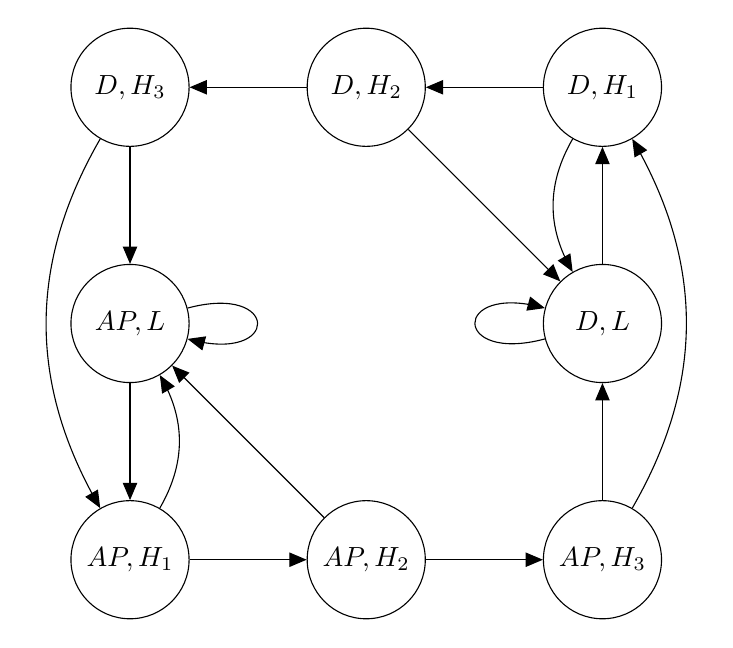
\begin{tikzpicture}[
        node distance=30mm,
        every node/.style={draw,circle,minimum size=1.5cm}
        ]
        \node[](apl) {$AP,L$};
        \node[below of=apl](aph1) {$AP,H_1$};
        \node[right of=aph1](aph2) {$AP,H_2$};
        \node[right of=aph2](aph3) {$AP,H_3$};
        \node[above of=aph3](dl) {$D,L$};
        \node[above of=dl](dh1) {$D,H_1$};
        \node[left of=dh1](dh2) {$D,H_2$};
        \node[left of=dh2](dh3) {$D,H_3$};
        \draw[->] (apl) -- (aph1);
        \draw[->] (aph1) -- (aph2);
        \draw[->] (aph2) -- (aph3);
        \draw[->] (aph3) -- (dl);
        \draw[->] (dl) -- (dh1);
        \draw[->] (dh1) -- (dh2);
        \draw[->] (dh2) -- (dh3);
        \draw[->] (dh3) -- (apl);
        \draw[->] (aph2) -- (apl);
        \draw[->] (dh2) -- (dl);
        \draw[->] (aph1) to[bend right] (apl);
        \draw[->] (dh3) to[bend right] (aph1);
        \draw[->] (apl) to[loop right] (apl);
        \draw[->] (dh1) to[bend right] (dl);
        \draw[->] (aph3) to[bend right] (dh1);
        \draw[->] (dl) to[loop left] (dl);
    \end{tikzpicture}
    \end{figure}

    Using the MDP above, we can produce a stationary distribution from it and
    the probabilities for a given TV's weight:

    \begin{figure}[H]
    \centering
    \begin{tabular}{|c||c|c|c|c|c|c|c|c|}
    \hline
    & $AP,L$ & $AP,H_1$ & $AP,H_2$ & $AP,H_3$ & $D,L$ & $D,H_1$ & $D,H_2$ &
    $D,H_3$ \\\hline\hline
    $AP,L$   & 0.467 & 0.533 & 0 & 0 & 0 & 0 & 0 & 0\\\hline
    $AP,H_1$ & 0.467 & 0 & 0.533 & 0 & 0 & 0 & 0 & 0\\\hline
    $AP,H_2$ & 0.467 & 0 & 0 & 0.533 & 0 & 0 & 0 & 0\\\hline
    $AP,H_3$ & 0 & 0 & 0 & 0 & 0.833 & 0.167 & 0 & 0\\\hline
    $D,L$    & 0 & 0 & 0 & 0 & 0.833 & 0.167 & 0 & 0\\\hline
    $D,H_1$  & 0 & 0 & 0 & 0 & 0.833 & 0 & 0.167 & 0\\\hline
    $D,H_2$  & 0 & 0 & 0 & 0 & 0.833 & 0 & 0 & 0.167\\\hline
    $D,H_3$  & 0.467 & 0.533 & 0 & 0 & 0 & 0 & 0 & 0\\\hline
    \end{tabular}
    \end{figure}
    Then, using the following formula for a stationary distribution, where $T$
    is the transition matrix from the previous part:
    $$ \pi = [1,0,\ldots,0]\cdot ((T-I)_1)^{-1} $$
    We would sum the probabilities for the TVs with anti-polka chips installed
    to get the expected value for the percentage of TVs that have anti-polka
    chips at the end of the day.
    \item{}
    We find $\pi$ to be:
    \begin{figure}[H]
    \centering
    \begin{tabular}{|c|c|c|c|c|c|c|c|}
    \hline
    $AP,L$ & $AP,H_1$ & $AP,H_2$ & $AP,H_3$ & $D,L$ & $D,H_1$ & $D,H_2$ &
    $D,H_3$ \\\hline\hline
    0.021 & 0.013 & 0.007 & 0.004 & 0.796 & 0.134 & 0.022 &  0.004\\\hline
    \end{tabular}
    \end{figure}
    Thus the expected value for the percentage of TVs that have anti-polka chips
    at the end of the day would be:
    $$ 0.021 + 0.013 + 0.007 + 0.004 = 0.045 \approx \textbf{4.5\%} $$
\end{enumerate}
\end{enumerate}

\end{document}
